% Options for packages loaded elsewhere
\PassOptionsToPackage{unicode}{hyperref}
\PassOptionsToPackage{hyphens}{url}
\PassOptionsToPackage{dvipsnames,svgnames,x11names}{xcolor}
%
\documentclass[
  letterpaper,
  DIV=11,
  numbers=noendperiod]{scrartcl}

\usepackage{amsmath,amssymb}
\usepackage{iftex}
\ifPDFTeX
  \usepackage[T1]{fontenc}
  \usepackage[utf8]{inputenc}
  \usepackage{textcomp} % provide euro and other symbols
\else % if luatex or xetex
  \usepackage{unicode-math}
  \defaultfontfeatures{Scale=MatchLowercase}
  \defaultfontfeatures[\rmfamily]{Ligatures=TeX,Scale=1}
\fi
\usepackage{lmodern}
\ifPDFTeX\else  
    % xetex/luatex font selection
\fi
% Use upquote if available, for straight quotes in verbatim environments
\IfFileExists{upquote.sty}{\usepackage{upquote}}{}
\IfFileExists{microtype.sty}{% use microtype if available
  \usepackage[]{microtype}
  \UseMicrotypeSet[protrusion]{basicmath} % disable protrusion for tt fonts
}{}
\makeatletter
\@ifundefined{KOMAClassName}{% if non-KOMA class
  \IfFileExists{parskip.sty}{%
    \usepackage{parskip}
  }{% else
    \setlength{\parindent}{0pt}
    \setlength{\parskip}{6pt plus 2pt minus 1pt}}
}{% if KOMA class
  \KOMAoptions{parskip=half}}
\makeatother
\usepackage{xcolor}
\setlength{\emergencystretch}{3em} % prevent overfull lines
\setcounter{secnumdepth}{-\maxdimen} % remove section numbering
% Make \paragraph and \subparagraph free-standing
\ifx\paragraph\undefined\else
  \let\oldparagraph\paragraph
  \renewcommand{\paragraph}[1]{\oldparagraph{#1}\mbox{}}
\fi
\ifx\subparagraph\undefined\else
  \let\oldsubparagraph\subparagraph
  \renewcommand{\subparagraph}[1]{\oldsubparagraph{#1}\mbox{}}
\fi

\usepackage{color}
\usepackage{fancyvrb}
\newcommand{\VerbBar}{|}
\newcommand{\VERB}{\Verb[commandchars=\\\{\}]}
\DefineVerbatimEnvironment{Highlighting}{Verbatim}{commandchars=\\\{\}}
% Add ',fontsize=\small' for more characters per line
\usepackage{framed}
\definecolor{shadecolor}{RGB}{241,243,245}
\newenvironment{Shaded}{\begin{snugshade}}{\end{snugshade}}
\newcommand{\AlertTok}[1]{\textcolor[rgb]{0.68,0.00,0.00}{#1}}
\newcommand{\AnnotationTok}[1]{\textcolor[rgb]{0.37,0.37,0.37}{#1}}
\newcommand{\AttributeTok}[1]{\textcolor[rgb]{0.40,0.45,0.13}{#1}}
\newcommand{\BaseNTok}[1]{\textcolor[rgb]{0.68,0.00,0.00}{#1}}
\newcommand{\BuiltInTok}[1]{\textcolor[rgb]{0.00,0.23,0.31}{#1}}
\newcommand{\CharTok}[1]{\textcolor[rgb]{0.13,0.47,0.30}{#1}}
\newcommand{\CommentTok}[1]{\textcolor[rgb]{0.37,0.37,0.37}{#1}}
\newcommand{\CommentVarTok}[1]{\textcolor[rgb]{0.37,0.37,0.37}{\textit{#1}}}
\newcommand{\ConstantTok}[1]{\textcolor[rgb]{0.56,0.35,0.01}{#1}}
\newcommand{\ControlFlowTok}[1]{\textcolor[rgb]{0.00,0.23,0.31}{#1}}
\newcommand{\DataTypeTok}[1]{\textcolor[rgb]{0.68,0.00,0.00}{#1}}
\newcommand{\DecValTok}[1]{\textcolor[rgb]{0.68,0.00,0.00}{#1}}
\newcommand{\DocumentationTok}[1]{\textcolor[rgb]{0.37,0.37,0.37}{\textit{#1}}}
\newcommand{\ErrorTok}[1]{\textcolor[rgb]{0.68,0.00,0.00}{#1}}
\newcommand{\ExtensionTok}[1]{\textcolor[rgb]{0.00,0.23,0.31}{#1}}
\newcommand{\FloatTok}[1]{\textcolor[rgb]{0.68,0.00,0.00}{#1}}
\newcommand{\FunctionTok}[1]{\textcolor[rgb]{0.28,0.35,0.67}{#1}}
\newcommand{\ImportTok}[1]{\textcolor[rgb]{0.00,0.46,0.62}{#1}}
\newcommand{\InformationTok}[1]{\textcolor[rgb]{0.37,0.37,0.37}{#1}}
\newcommand{\KeywordTok}[1]{\textcolor[rgb]{0.00,0.23,0.31}{#1}}
\newcommand{\NormalTok}[1]{\textcolor[rgb]{0.00,0.23,0.31}{#1}}
\newcommand{\OperatorTok}[1]{\textcolor[rgb]{0.37,0.37,0.37}{#1}}
\newcommand{\OtherTok}[1]{\textcolor[rgb]{0.00,0.23,0.31}{#1}}
\newcommand{\PreprocessorTok}[1]{\textcolor[rgb]{0.68,0.00,0.00}{#1}}
\newcommand{\RegionMarkerTok}[1]{\textcolor[rgb]{0.00,0.23,0.31}{#1}}
\newcommand{\SpecialCharTok}[1]{\textcolor[rgb]{0.37,0.37,0.37}{#1}}
\newcommand{\SpecialStringTok}[1]{\textcolor[rgb]{0.13,0.47,0.30}{#1}}
\newcommand{\StringTok}[1]{\textcolor[rgb]{0.13,0.47,0.30}{#1}}
\newcommand{\VariableTok}[1]{\textcolor[rgb]{0.07,0.07,0.07}{#1}}
\newcommand{\VerbatimStringTok}[1]{\textcolor[rgb]{0.13,0.47,0.30}{#1}}
\newcommand{\WarningTok}[1]{\textcolor[rgb]{0.37,0.37,0.37}{\textit{#1}}}

\providecommand{\tightlist}{%
  \setlength{\itemsep}{0pt}\setlength{\parskip}{0pt}}\usepackage{longtable,booktabs,array}
\usepackage{calc} % for calculating minipage widths
% Correct order of tables after \paragraph or \subparagraph
\usepackage{etoolbox}
\makeatletter
\patchcmd\longtable{\par}{\if@noskipsec\mbox{}\fi\par}{}{}
\makeatother
% Allow footnotes in longtable head/foot
\IfFileExists{footnotehyper.sty}{\usepackage{footnotehyper}}{\usepackage{footnote}}
\makesavenoteenv{longtable}
\usepackage{graphicx}
\makeatletter
\def\maxwidth{\ifdim\Gin@nat@width>\linewidth\linewidth\else\Gin@nat@width\fi}
\def\maxheight{\ifdim\Gin@nat@height>\textheight\textheight\else\Gin@nat@height\fi}
\makeatother
% Scale images if necessary, so that they will not overflow the page
% margins by default, and it is still possible to overwrite the defaults
% using explicit options in \includegraphics[width, height, ...]{}
\setkeys{Gin}{width=\maxwidth,height=\maxheight,keepaspectratio}
% Set default figure placement to htbp
\makeatletter
\def\fps@figure{htbp}
\makeatother
\newlength{\cslhangindent}
\setlength{\cslhangindent}{1.5em}
\newlength{\csllabelwidth}
\setlength{\csllabelwidth}{3em}
\newlength{\cslentryspacingunit} % times entry-spacing
\setlength{\cslentryspacingunit}{\parskip}
\newenvironment{CSLReferences}[2] % #1 hanging-ident, #2 entry spacing
 {% don't indent paragraphs
  \setlength{\parindent}{0pt}
  % turn on hanging indent if param 1 is 1
  \ifodd #1
  \let\oldpar\par
  \def\par{\hangindent=\cslhangindent\oldpar}
  \fi
  % set entry spacing
  \setlength{\parskip}{#2\cslentryspacingunit}
 }%
 {}
\usepackage{calc}
\newcommand{\CSLBlock}[1]{#1\hfill\break}
\newcommand{\CSLLeftMargin}[1]{\parbox[t]{\csllabelwidth}{#1}}
\newcommand{\CSLRightInline}[1]{\parbox[t]{\linewidth - \csllabelwidth}{#1}\break}
\newcommand{\CSLIndent}[1]{\hspace{\cslhangindent}#1}

\usepackage{booktabs}
\usepackage{longtable}
\usepackage{array}
\usepackage{multirow}
\usepackage{wrapfig}
\usepackage{float}
\usepackage{colortbl}
\usepackage{pdflscape}
\usepackage{tabu}
\usepackage{threeparttable}
\usepackage{threeparttablex}
\usepackage[normalem]{ulem}
\usepackage{makecell}
\usepackage{xcolor}
\KOMAoption{captions}{tableheading}
\makeatletter
\makeatother
\makeatletter
\makeatother
\makeatletter
\@ifpackageloaded{caption}{}{\usepackage{caption}}
\AtBeginDocument{%
\ifdefined\contentsname
  \renewcommand*\contentsname{Innholdsfortegnelse}
\else
  \newcommand\contentsname{Innholdsfortegnelse}
\fi
\ifdefined\listfigurename
  \renewcommand*\listfigurename{Figuroversikt}
\else
  \newcommand\listfigurename{Figuroversikt}
\fi
\ifdefined\listtablename
  \renewcommand*\listtablename{Tabelloversikt}
\else
  \newcommand\listtablename{Tabelloversikt}
\fi
\ifdefined\figurename
  \renewcommand*\figurename{Figur}
\else
  \newcommand\figurename{Figur}
\fi
\ifdefined\tablename
  \renewcommand*\tablename{Tabell}
\else
  \newcommand\tablename{Tabell}
\fi
}
\@ifpackageloaded{float}{}{\usepackage{float}}
\floatstyle{ruled}
\@ifundefined{c@chapter}{\newfloat{codelisting}{h}{lop}}{\newfloat{codelisting}{h}{lop}[chapter]}
\floatname{codelisting}{Liste}
\newcommand*\listoflistings{\listof{codelisting}{Listeoversikt}}
\makeatother
\makeatletter
\@ifpackageloaded{caption}{}{\usepackage{caption}}
\@ifpackageloaded{subcaption}{}{\usepackage{subcaption}}
\makeatother
\makeatletter
\@ifpackageloaded{tcolorbox}{}{\usepackage[skins,breakable]{tcolorbox}}
\makeatother
\makeatletter
\@ifundefined{shadecolor}{\definecolor{shadecolor}{rgb}{.97, .97, .97}}
\makeatother
\makeatletter
\makeatother
\makeatletter
\makeatother
\ifLuaTeX
  \usepackage{selnolig}  % disable illegal ligatures
\fi
\IfFileExists{bookmark.sty}{\usepackage{bookmark}}{\usepackage{hyperref}}
\IfFileExists{xurl.sty}{\usepackage{xurl}}{} % add URL line breaks if available
\urlstyle{same} % disable monospaced font for URLs
\hypersetup{
  pdftitle={Arbeidskrav},
  colorlinks=true,
  linkcolor={blue},
  filecolor={Maroon},
  citecolor={Blue},
  urlcolor={Blue},
  pdfcreator={LaTeX via pandoc}}

\title{Arbeidskrav}
\author{}
\date{}

\begin{document}
\maketitle
\ifdefined\Shaded\renewenvironment{Shaded}{\begin{tcolorbox}[sharp corners, breakable, frame hidden, borderline west={3pt}{0pt}{shadecolor}, interior hidden, boxrule=0pt, enhanced]}{\end{tcolorbox}}\fi

Formålet og motivasjonen for denne artikkelen er å se på mulige
pådrivere som påvirker by-land-skillet i Europa. For å belyse dette skal
vi kritisk undersøke hvordan faktorer påvirker by-land-skillet slik som
arbeidsledighetsraten, sysselsettingsvekst og det lokale boligmarkedet
påvirker mønstrene for befolkningsfordelingen og jobbskapingen på tvers
av ulike europeiske land. Dataene som er benyttet i denne studien er
nøye samlet inn fra Eurostat ({``Database - {Eurostat}''} n.d.), som er
en pålitelig kilde for europeisk statistikk og økonomisk informasjon. Vi
har spesifikt fokusert på andelene av den totale arbeidskraften til
hvert land, som presenteres grundig gjennom Eurostats rapporter. For å
kunne trekke konklusjoner og utføre en grundig analyse har vi valgt å
sammenligne land som vi mener er best egnet for å belyse vår hypotese.
Disse landene inkluderer Østerrike, Belgia, Tyskland, Danmark, Estland,
Hellas, Spania, Finland, Frankrike, Irland, Italia, Luxembourg, Norge,
Nederland, Polen, Portugal, Sverige, Slovenia, og Slovakia. Ved å ta i
betraktning denne omfattende og varierte gruppen av land, sikter vi mot
å få et dyptgående innblikk i de dynamiske kreftene bak by-land-skillet
i Europa.

\hypertarget{litteraturgjennomgang}{%
\subsection{Litteraturgjennomgang}\label{litteraturgjennomgang}}

Manuel Wolff (2018) beskriver den økende polariseringen av både
sentraliserende og desentraliserende voksende byer, samt en trend mot
sentralisert tilbakegang. Dette fenomenet peker på behovet for ulike
planleggingstiltak. Samtidig påpekes det at omlandet mister betydning,
spesielt for synkende byer (Wolff 2018).

Urbanisering er et fenomen som i økende grad påvirker økonomier,
samfunn, kulturer og miljøet. Ifølge OECD og Europakommisjonen (2020)
forventes det at 55 \% av verdens befolkning vil bo i byer innen 2050.
Denne veksten i bybefolkningen har skapt økt interesse for både den
raske utviklingen og formen på urbane områder, samt for de tette båndene
som eksisterer mellom individuelle byer og mellom byer og landlige
områder. En spesifikk politisk interesse retter seg mot megabyer og
store metropolområder som drar nytte av agglomerasjon, industrielle
klynger og innovasjon, men som samtidig står overfor betydelige
utfordringer knyttet til bærekraftig byutvikling, for eksempel
trafikkork eller miljøpåvirkninger (European Commission. Statistical
Office of the European Union. 2021).~

Samtidig viser forskning at ulikhetene mellom urbane og rurale områder
synes å minske. Gjennom hierarkiske lineære regresjonsmodeller avdekkes
det at inaktivitet øker både i urbane og rurale områder, selv om den er
høyere i sistnevnte. Denne økningen bidrar til å redusere den
urbane-rurale forskjellen og eliminerer den til og med i noen land.
Dette fenomenet kan peke i retning av en økning i forstedene (suburbs),
da det ser ut til å være en tendens til at de urbane og rurale
karakterene blir mer like (Moreno-Llamas, García-Mayor, and De la
Cruz-Sánchez 2021).

På den andre siden står indre periferier i EU overfor betydelige
utfordringer. Disse områdene, som utgjør over 45 \% av det europeiske
territoriet, lider av periferi- og marginalitetsforhold. De har dårlig
tilgang til generelle tjenester, lavt økonomisk potensial på grunn av
avstand til sentre for økonomisk aktivitet, og mangler relasjonell
nærhet til maktsentre, noe som hindrer lokalsamfunnets aktive deltakelse
i utviklingspolitikk. Dette fører til demografisk tilbakegang, høy
arbeidsledighet, sosial ekskludering, tap av lokal identitet og følgelig
til nedlagte områder (De Toni, Di Martino, and Dax 2021).

\hypertarget{faktorer-som-puxe5virker-befolkningsvekst}{%
\subsection{\texorpdfstring{\textbf{Faktorer som påvirker
befolkningsvekst}}{Faktorer som påvirker befolkningsvekst}}\label{faktorer-som-puxe5virker-befolkningsvekst}}

I dette delkapittelet vil vi utforske ulike faktorer som påvirker
befolkningsvekst. Videre vil rapporten presentere tre teorier - budrente
teorien, shift-share-analyse og Williamson's inverterte U - og vurdere i
hvilken grad de beskriver og forklarer trender i befolkningsvekst.
Grunnet mangelfull data vil anvendelsen av teoriene benyttes i form av
momenter som beskrivende faktorer for om befolkningsveksten i de
overordnete valgte europeiske landene har en tendens til sentralisering
eller desentralisering.

Med utgangspunkt i budrenteteorien er det to faktorer som avgjør hvor
befolkningen bosetter seg i form av r (pris på bolig/rentekostnader) og
distanse fra sentrum. Ettersom litteraturen viser til en større grad av
teknologisk fremskritt på landsnivå, danner dette grunnlaget for at man
ikke har et grunnleggende behov for å bo i sentrum for å kunne ta nytte
av teknologien som er i sentrum. «Sentralisering til byene bidrar til
økt press på boliger og priser. Det kan dermed være billigere å anskaffe
leiligheter som er lokalisert i områder utenfor sentrum med lavere
tetthet'' (Christiansen and Loftsgarden 2011, s. 2) og danner grunnlag
for en økt grad av desentralisering da befolkningen får «mer for
pengene» ved økt distanse til sentrum. Det er allikevel viktig å
presisere at budrenteteorien har en bedre anvendelse på et bynivå og
fungerer dårlig på landsnivå, men vil heller i prinsipp danne grunnlaget
som et moment for desentralisering.

Shift - share - analyse er en økonomisk analysemetode som benyttes til å
forstå veksten eller endringen i en bransje, økonomi, eller i dette
tilfellet en endring i regionale veksthastigheter. I det tilgjengelige
datamaterialet fra Eurostat vil å gjennomføre denne analysen ikke
inneholde tilstrekkelig med data da ``Den grunnleggende ideen for å
beskrive regionale veksthastigheter påvirkes dette av tre faktorer i
form av'' (Capello 2015, s. 106) ;

\begin{itemize}
\item
  Den industrielle strukturen: Denne faktoren referer til
  sammensettingen av næringer eller sektorer i en bestemt region.
\item
  Sektorens produktivitet: Produktiviteten til en sektor eller næring
  indikerer effektiviteten til produksjonsprosessen, hvor en økning i
  effektiviteten vil bidra positivt til den totale veksten.
\item
  Dynamikken i etterspørsel og forbrukerpreferanser: Endringer i
  etterspørsel og forbrukerpreferanser påvirker hvilke varer og
  tjenester som etterspør. Den avgjørende faktoren her vil være i hvor
  stor grad regionen er kapabel til å tilpasse seg endringer.

  Man skiller shift-share-analysen i å bestå av Differensiell effekter
  (konkurransedyktighet) og Mix-effekter (Etterspørsel) som grunnlag for
  i hvilken grad en region gjør det bedre enn andre regioner i et land.
  Det kommer frem av tidligere forskning at sentrale områder har større
  konkurransekraft og vil da danne et grunnlag for at en
  shift-share-analysen er et moment for sentralisering. (Christiansen
  and Loftsgarden 2011)
\end{itemize}

På midten av 1960-tallet presenterte Williamson sin teori om regionale
utviklingsfaser og forskjeller i et land. Teorien gikk ut på at
utvikling er konsentrert og polarisert i de tidlige stadiene, før den
senere sprer seg til mer perifere områder (suburb, og rurale områder).
Dette gir en kurve formet som en invertert U.

Årsakene til de økende ulikhetene er; (1) utvandring av kompetent
arbeidskraft fra svake til sterke områder, (2) kapitalstrøm til de
rikere regionene, tiltrukket av høyere etterspørsel, tilgjengelighet av
infrastruktur, tjenester, et potensielt marked og bedre miljøforhold for
bedrifter, (3) allokering av en større del av offentlige investeringer
til sterke områder, som svar på etterspørsel, og (4) begrenset handel
mellom regioner, slik at i de tidlige stadiene utøver ikke de rike
regionene trekkraft på det fattige (Capello 2015, s. 105).

Til slutt vises mekanismer som virker i motsatt retning som fører til
mindre ulikheter; (1) skaping av nye jobber i mindre utviklede regioner,
med den konsekvensen at utvandring avtar eller til og med stopper opp,
(2) klyngeulemper, som f.eks. høye boligpriser, forurensing, trafikk og
bråk, (3) vekst i offentlige investeringer i svake områder, og (4)
begynnelsen av trekkraft utøvet av det sterke området på det svake
(Capello 2015, s. 105).

\hypertarget{hypotese}{%
\subsubsection{Hypotese}\label{hypotese}}

Ut i fra budrenteteorien velger befolknigen hvor de vil bosette seg i
form av betalingsvillighet og distanse fra sentrum. Ettersom
litteraturen viser til en større grad av teknologisk fremskritt på
landsnivå, taler dette for at vi vil gjerne få en desentralisering av
samfunnet, ettersom det er mindre trykk på boligprisen. Merknad;
budrenteteorien har en bedre anvendelse på et bynivå og fungerer i
dårligere grad på landsnivå, allikvel mener vi at prinsippet danner
grunnlaget for en hypotese om desentralisering. Ser man på shift - share
- analysen danner denne grunnlag for en sentralisering i
befolkningsutviklingen.

Både litteraturen og teorien sett i lys av hverandre danner grunnlag for
en hypotese om desentralisering.

\hypertarget{data-analyse}{%
\subsubsection{\texorpdfstring{\textbf{Data-analyse:}}{Data-analyse:}}\label{data-analyse}}

For å se nærmere på by-land-skillet trekker vi ut 3 underkatogorier av
variabelen `Region Type' i form av;~

\begin{itemize}
\item
  City (tett befolkede områder)
\item
  Suburb (områder med middels tetthet)
\item
  Rurale områder (tynt befolkede områder)
\end{itemize}

Vi skal nå analysere befolkningsveksttrender ved hjelp av disse
kategoriene.~

\begin{figure}

{\centering 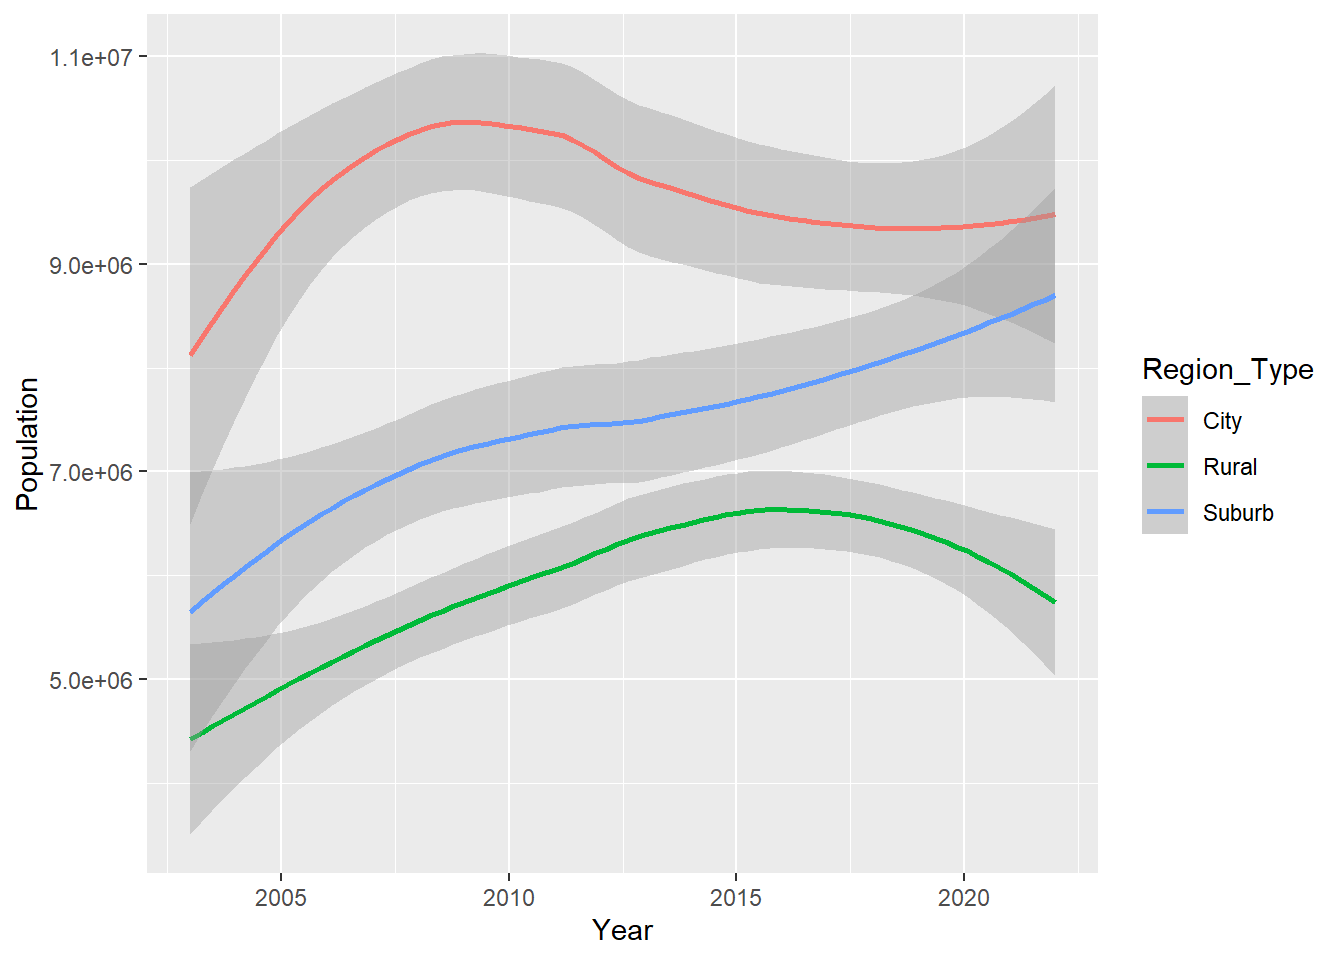
\includegraphics{assignment_files/figure-pdf/fig-1-1.pdf}

}

\caption{\label{fig-1}Befolkningsvekst for ulike regioner i perioden
2003-2022}

\end{figure}

\protect\hyperlink{fig-1}{Figur 1} viser gjennomsnittlig
befolkningsvekst for de tre ulike regiontypene fra 2003 til 2022. Vi ser
en trend i befolkningsutviklingen frem til 2010 at byer har en markant
størst vekst, dette kan forklares ved hjelp av momentet i
shift-share-analysen om at byer har en størst konkurransekraft og
effektivitet gjennom klyngefordeler som kjennetegner å være i sentrum.
Det vil også være en nærliggende forklaring at dynamikken mellom
etterspørsel og forbruker preferanser skiller byer seg spesielt ut til å
være kapabel til å tilpasse seg endringer ettersom sentrum gjerne
kjennetegnes for å være ressurssterke, som fører til en sentralisering
av samfunnet frem til 2010. For resterende del av perioden trender i
befolkningsveksten til en gradvis reduksjon av befolkningen i byer fra
2010 til 2016, før den flater ut i perioden 2017-2022. Forklaringen på
dette kan være at nedgangen skyldes budrenteteorien med hensyn på
desentralisering, teknologiskutvikling og «spillovers» fra regions typen
«city» til «suburb».

Av Figur~\ref{fig-1} ser man at suburb-regioner har en tendens til å ha
en kontinuerlig vekst i perioden. Forklaringen på dette kan være med
hensyn på shift-share. Dette er den regiontypen som ligger tettes opp
mot byer og vil ved hjelp av momenter i shift-share-analysen som
teknologisk utvikling kan i denne sammenheng tolkes til å være
utviklingen i i infrastuktur, som veinett og jernbane. Dette fører til
økt effektivitet, hvor suburb drar nytte av spillovers fra byer. Et
annet moment i budrenteteorien er at ved det økte presset vi så
befolkningsveksten i byer frem til 2010, føre til at det er mer gunstig
for befolkningen å bosette seg i suburbs, som drar i retning av
desetralisering.

Vi ser en trend i befolkningsveksten fra 2016 til 2022 en markant
nedgang i rurale områder. Forklaringen på dette kan være
sentralitets/periferitets-tilnærmingen, som betrakter avstanden fra
sentrum av økonomiske aktiviteter som årsaken til forsinket utvikling.
Den påpeker at geografisk sentralitet i seg selv er en faktor som
fremmer utvikling, mens periferi hindrer det. Faktorer som avgjør dette
er; (1) tilgang til informasjon, (2) teknologisk kunnskap, (3)
tilgjengeligheten av markedene for varer og produksjonsfaktorer, (4)
transportkostnader for ferdige varer, råvarer og halvfabrikata, og (5)
forsinkelser i adopsjonen av innovasjoner (Capello 2015, s. 111).

Teorien om ``The spatial diffusion of innovation'' kan også være en
mulig forklaring, som fokuserer på at distansen fra sentrale områder er
en viktig del av teknologisk utvikling (Capello 2015, s. 188). Flytter
man langt fra sentrum vil en gradvis falle bak utviklingen og som
Capello gjorde kjent, vil det å vente med å ta i bruk ny teknologi koste
mer jo lengre en venter (Capello 2015).

Gjennom momenter fra budrenteteorien og shift-share-analyse ved støtte
fra litteraturen, ser man av Figur~\ref{fig-1} en klar tendens til
desentralisering fra ``City'' til ``Suburb'' ettersom man ser en økt
teknologisk utvikling i Europa og et ekstremt press på boligmarkedet,
som vil føre til en desentralisering.

Vi vil videre bruke 2005 som et indeksår, som definerer befolkningen til
å være 100 i 2005. Dette er på grunn av manglende observasjoner for år
2003 og 2004. Dermed representerer kurvene prosentvis befolkningsvekst
over den aktuelle perioden 2005 til 2022.

Videre skal vi utforske variasjoner for ulike europeiske land. Vi har
gjort dette ved å dele utvalget av land fra Eurostat inn i tre
hovedgrupper; urbaniserte land, mellomstore bosettingsland og rurale
land. Inndelingen er basert på bosettingsmønster for alle landene i
datasettet, hvor vi har gruppert de landene som har lignende utvikling,
se \protect\hyperlink{fig-9}{Figur 9} i appendix.

Gruppe 1, urbaniserte land, består av Østerrike (AT), Belgia (BE),
Tyskland (DE), Danmark (DK), Spania (ES), Finland (FI), Frankrike (FR),
Italia (IT) og Nederland (NL). Gruppe 2, mellomstore bosettingsland,
består av Irland (IE), Norge (NO) og Sverige (SE). Gruppe 3, rurale
land, består av Polen (PL), Portugal (PT), Slovenia (SI) og Slovakia
(SK).

Innenfor de nevnte gruppene av land synes det å være visse likheter i
urbaniseringsmønstre og økonomiske strukturer, sannsynligvis påvirket av
geografiske og kulturelle faktorer. F.eks. deler landene i Gruppe 1, som
Tyskland, Frankrike og Italia, lignende urbaniseringsmønstre og
økonomiske strukturer på grunn av sin nærhet og felles historie.
Tilsvarende kan landene i Gruppe 3, som Polen og Slovakia, dele lignende
utfordringer med rurale karakterer og tidligere kommunistisk historie.
Gruppe 2 viser imidlertid mer variasjon; Norge har en betydelig
spredning av befolkning i mindre byer og spredtbygde områder, mens
Irland og Sverige har mer markante bymessige og forstedlige (suburb)
bosettingsmønstre.

\textbf{Gruppe 1: Urbaniserte land}

\begin{figure}

{\centering 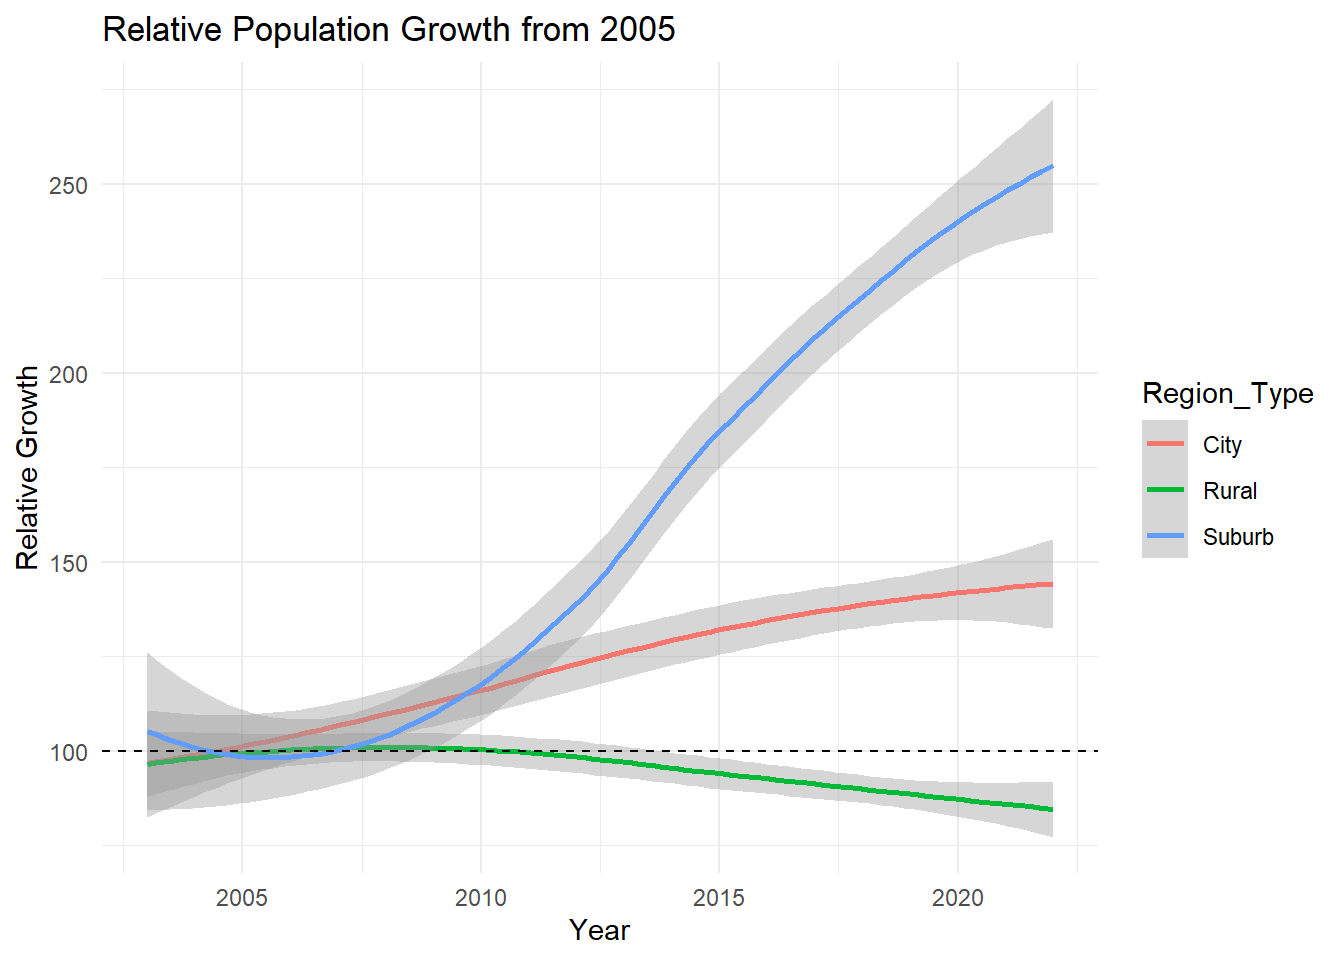
\includegraphics{assignment_files/figure-pdf/fig-3-1.pdf}

}

\caption{\label{fig-3}Relativ befolkningsvekst gruppe 1}

\end{figure}

\protect\hyperlink{fig-3}{Figur 3} viser gjennomsnittlig relativ
befolkningsvekst for de tre ulike regiontypene fra 2005 til 2022 for
gruppe 1, og har en tendens til desentralisering hvor folk bosetter seg
hovedsakelig i rurale områder og suburbs. Dette kan tyde på at det har
vært et høyt press på boligpriser i disse landene, hvor man gjennom
budrenteteorien som prinsipp for land velger å bosette seg utenfor
sentrale områder.

\textbf{Gruppe 2: Mellomstore bosettingsland}

\begin{figure}

{\centering 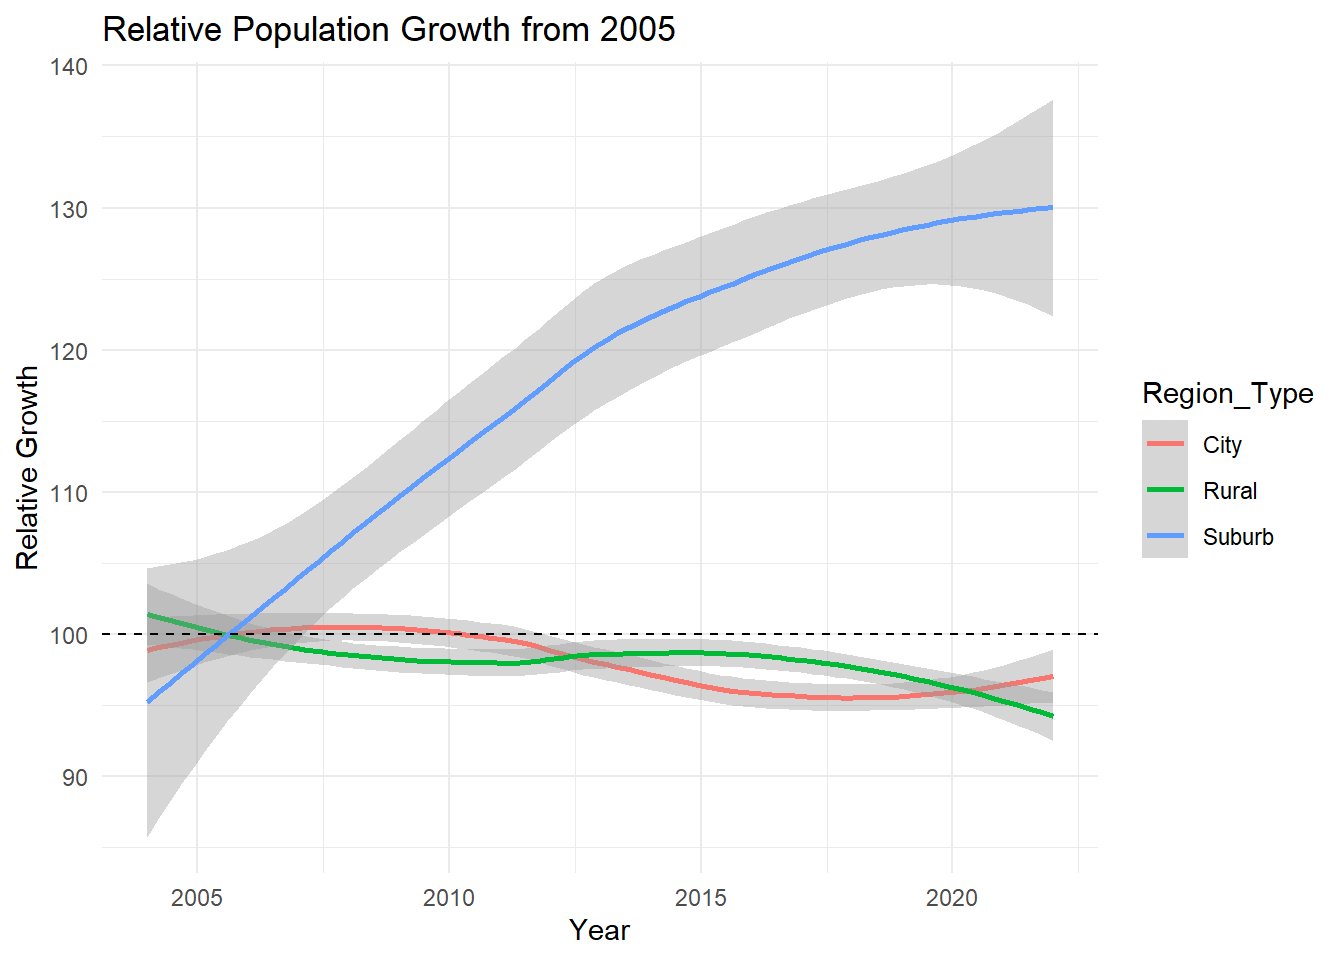
\includegraphics{assignment_files/figure-pdf/fig-4-1.pdf}

}

\caption{\label{fig-4}Relativ befolkningsvekst gruppe 2}

\end{figure}

\protect\hyperlink{fig-4}{Figur 4} viser en gjennomsnittlig relativ
befolkningsvekst for de tre ulige regiontypene fra 2005 til 2022 for
gruppe 2, hvor man ser en tendens i befolkningsutviklingen at man
bosetter seg i ``suburbs'' og ``city''. Ettersom man i gruppe 2 har en
størst befolkningsvekt i suburb og en kontunuerlig vekst i byer kan
forklaringen på dette skyldes at man har en spillover effekt fra byer
til suburbs med teknologisk utvikling, samt man har en prinsippielt
lavere boligpris ved bosettelse i suburb. Nedgangen i rural kan skyldes
forsinket utvikling i rurale områder i henhold til
sentralitets/periferitets-tilnærmingen.

\textbf{Gruppe 3: Rurale land}

\begin{figure}

{\centering 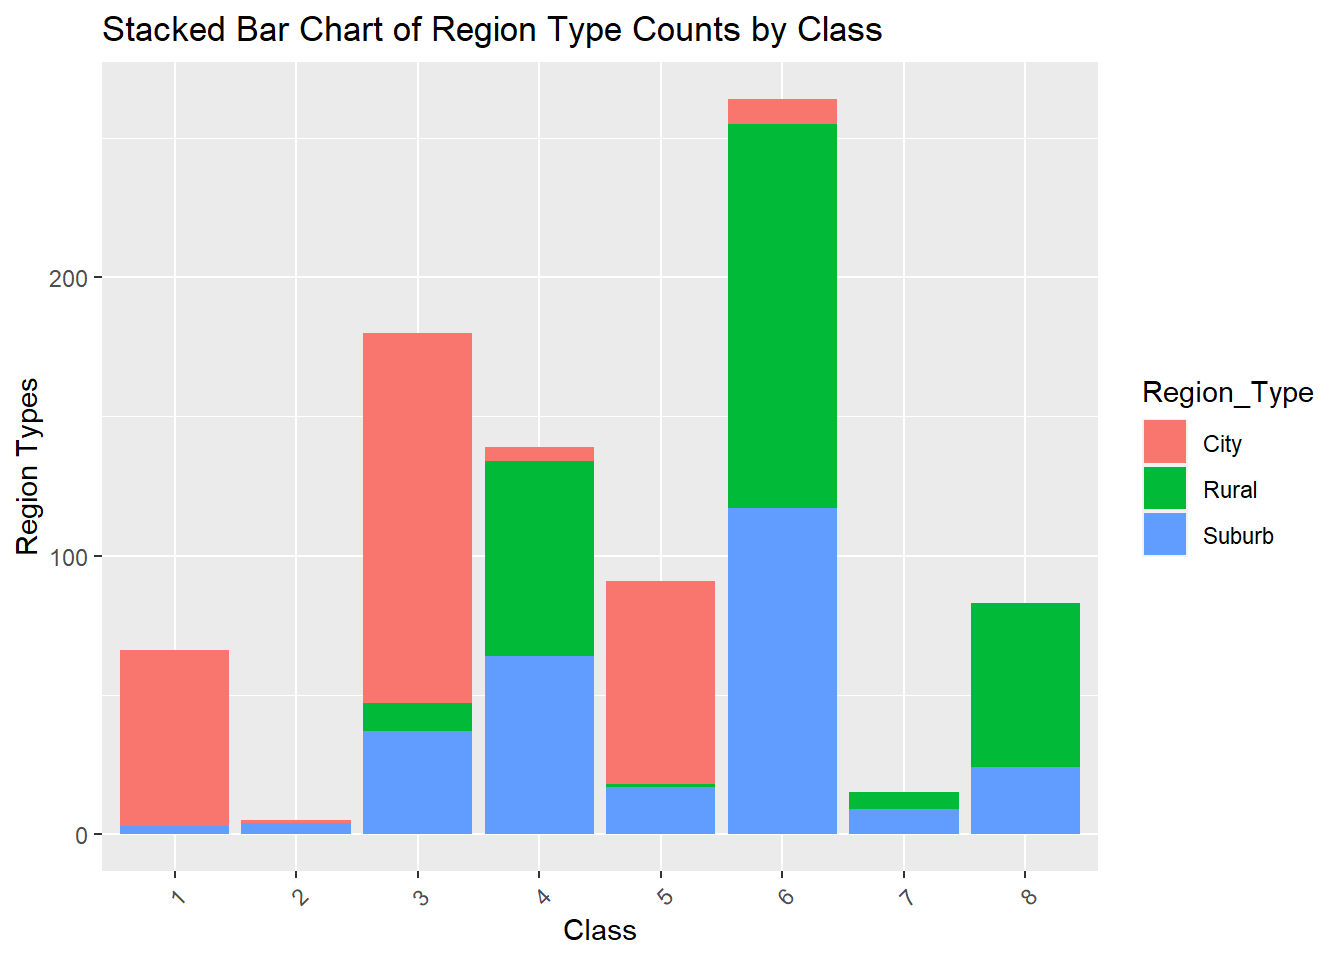
\includegraphics{assignment_files/figure-pdf/fig-5-1.pdf}

}

\caption{\label{fig-5}Relativ befolkningsvekst gruppe 3}

\end{figure}

\protect\hyperlink{fig-5}{Figur 5} viser en gjennomsnittlig relativ
befolkningsvekst for de tre ulige regiontypene fra 2005 til 2022 for
gruppe 3. Man ser her at den eneste regoinstypen som har hatt en positiv
vekst i befolkningsutviklingen er suburb. Dette skyldes nok en støtte
grad av spillover med teknologisk utvikling og et større press på
boligpriser enn gruppe 2, som fører til en desentralisering av
samfunnet.

\hypertarget{forstuxe5-uxf8konomiske-faktorer-som-puxe5virker-befolkningsvekst}{%
\subsection{\texorpdfstring{\textbf{Forstå økonomiske faktorer som
påvirker
befolkningsvekst}}{Forstå økonomiske faktorer som påvirker befolkningsvekst}}\label{forstuxe5-uxf8konomiske-faktorer-som-puxe5virker-befolkningsvekst}}

For å fortsette oppgaven, har vi laget oss 8 forskjellige grupper basert
på tre kriterium: arbeidsledighet (U), sysselsettingsvekst (∆E) og
boligpriser (H); disse gruppene er basert på arbeidet av (Andersson,
Håkansson, and Thorsen 2019). Ved å se på disse gruppene, og sammenligne
dem med city, suburb og rurale områder, kan vi undersøke
sentraliseringstrender over tid, samt få en dypere forståelse av
regionenes økonomiske dynamikk. De 8 gruppene kan også gi oss et mer
nyansert bilde av økonomisk vekst og boligmarkedstrender, ved å tilby en
mer differensiert analyse av regionale utviklingsmønstre enn hva det å
kun se på city, suburb og rurale områder kan gi oss. Gruppene er delt
inn i følgende format:

\begin{enumerate}
\def\labelenumi{\arabic{enumi}.}
\tightlist
\item
  Høy U, høy ∆E og høy H
\item
  Høy U, høy ∆E og lav H
\item
  Høy U, lav ∆E og høy H
\item
  Høy U, lav ∆E og lav H
\item
  Lav U, høy ∆E og høy H
\item
  Lav U, høy ∆E og lav H
\item
  Lav U, lav ∆E og høy H
\item
  Lav U, lav ∆E og lav H
\end{enumerate}

Bestemmelsene for om verdiene er høye eller lave er basert på den
relative størrelsen målt opp mot det samledet gjennomsnittet av alle
land. En forutsetning for økonomisk vekst i en region er en høy
boligpris ettersom dette reflekterer et attraktivt området som under
vekst. Kategoriene 1-6 og 8 er høyst vektet av byer og viser en trend
til sentralisering rundt bykjernen. Kategori 7 har flest suburb og
rurale regioner med høy boligpris, og viser i andre retning mot en
desentralisering.

\hypertarget{avgjuxf8rende-faktorer-som-danner-grunnlaget-for-uxe5-forstuxe5-befolkningsutviklingen}{%
\subsubsection{Avgjørende faktorer som danner grunnlaget for å forstå
befolkningsutviklingen}\label{avgjuxf8rende-faktorer-som-danner-grunnlaget-for-uxe5-forstuxe5-befolkningsutviklingen}}

1.\textbf{Eb (Basissektoren):} Basissektoren består av bransjer eller
aktiviteter som er rettet mot eksterne markeder, for eksempel
eksportindustrier. Økningen eller reduksjonen i sysselsettingen innen
basissektoren kan ha betydelige ringvirkninger på den totale økonomien
og dermed på befolkningsutviklingen.

2. \textbf{ACC (Tilgjengelighet):} Tilgjengelighet er ofte en viktig
faktor for befolkningsutviklingen. Dette kan referere til
tilgjengeligheten av transportinfrastruktur, veier, kollektivtransport
eller annen infrastruktur som gjør det lettere for folk å komme til og
fra området. Bedre tilgjengelighet kan tiltrekke flere innbyggere.

3.\textbf{Shopping (Handelsmuligheter):} Handelsmuligheter, som
tilgjengeligheten av butikker og handelssentre, kan også påvirke
befolkningsutviklingen. Et område med et variert og tilfredsstillende
handelstilbud kan tiltrekke seg innbyggere og bidra til vekst.

4. \textbf{Amenity (Bekvemmeligheter):} Ameniteter refererer til
fasiliteter eller bekvemmeligheter i et område som øker livskvaliteten.
Dette kan inkludere parker, rekreasjonsområder, kulturelle fasiliteter,
og andre elementer som gjør området mer attraktivt å bo i. Gode
ameniteter kan være en lokkende faktor for befolkningsvekst.

Disse faktorene representerer ulike dimensjoner av det sosioøkonomiske
miljøet i en region, og sammen kan de bidra til å skape et attraktivt
miljø som påvirker befolkningsutviklingen positivt (Capello 2015).

\begin{figure}

{\centering 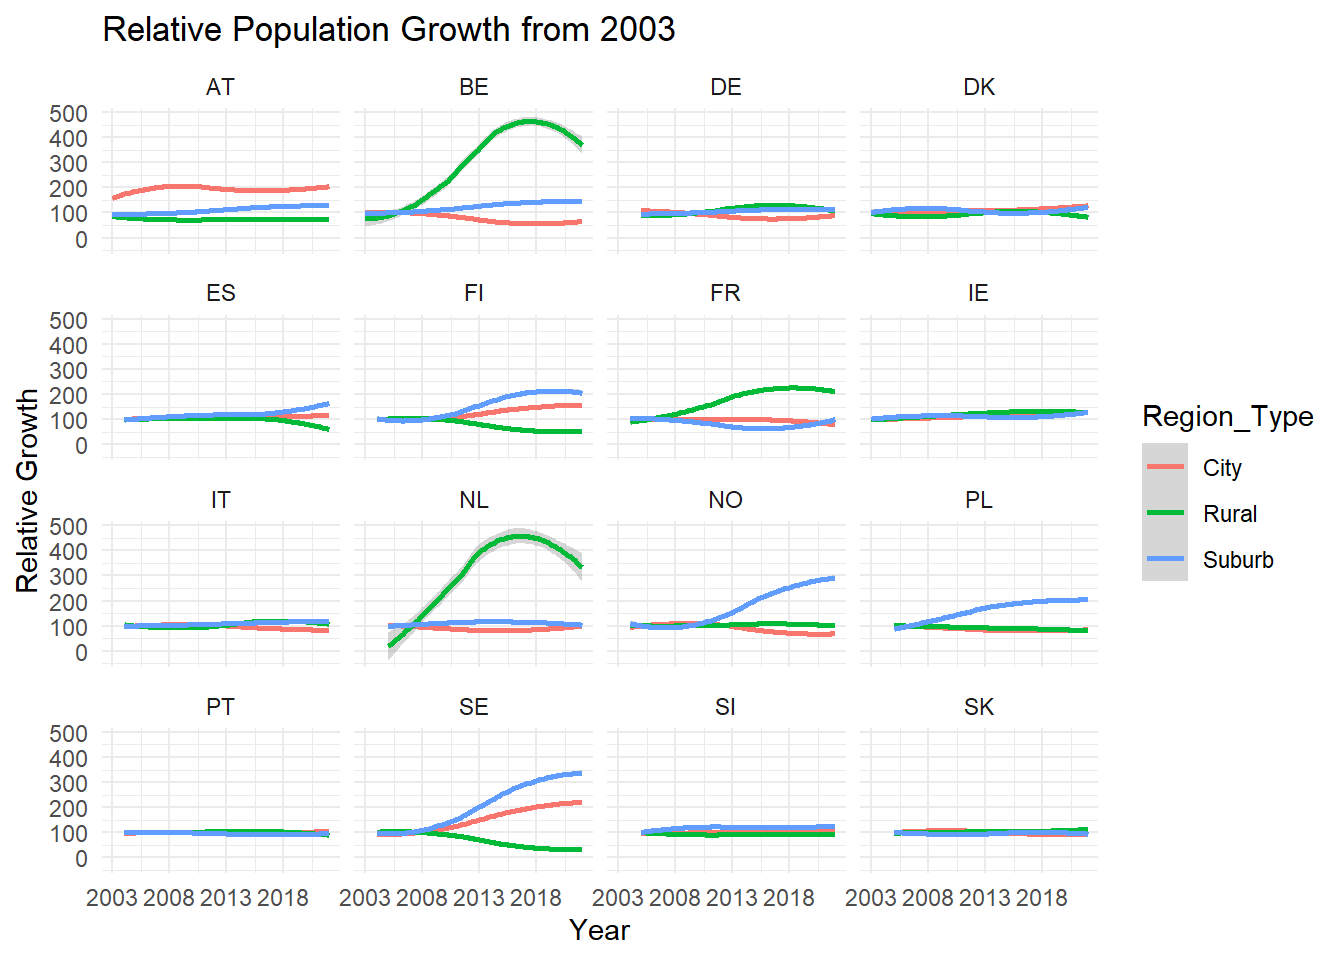
\includegraphics{assignment_files/figure-pdf/fig-6-1.pdf}

}

\caption{\label{fig-6}Regiontyper gruppert etter grupper}

\end{figure}

\protect\hyperlink{fig-6}{Figur 6} illustrerer variasjonen i geografiske
områder basert på arbeidsledighet (U), sysselsettingsvekst (ΔE), og
boligpriser (H). Kategori 1, 3 og 5 er dominert av byer. Det som
kjennetegner en by på sysselsetting er at det er bredt spekter av
jobbmuligheter over ulike sektorer, hvor det er tilstedeværelse av store
bedrifter og næringsliv. Byer har i utgangspunktet en lav
arbeidsledighet pga. tilgang på varierte jobbmuligheter og høyt
aktivitetsnivå. Imidlertid kan konkurransen for enkelte type stillinger
føre til at spesifikke bransjer opplever høy arbeidsledighet. Det er en
tendens til at boligprisene er høye ettersom arbeidsplasser ligger nærme
arbeidsplasser, utdanningsinstitusjoner og kulturelle fasiliteter.
Konkurransen om boliger kan drive prisen opp og tilbudet vil være
begrenset.

Kategori 2, 4 og 7 domineres av suburbs, og er ofte preget av et mer
variert arbeidsliv med mindre bedrifter og i noen tilfeller
industriområder. Hvordan sysselsettingen er kan påvirkes av
tilknytningen til byer og tilgjengeligheten til arbeidsplasser.
Boligprisene varierer ut ifra tilgangen til byen.~

Kategori 6 og 8 er preget av rural, hvor det er begrenset med jobber som
finnes, og de er gjerne dominert av jordbruk, skogbruk og fiske.
Muligheten for jobbdifferensiering kan være begrenset her.
Arbeidsledigheten avhenger av de økonomiske aktivitetene i området, og
sesongmessig arbeidsledighet kan være relevant. Boligprisene har en
tendens til å være lavere sammenlignet med byer og suburb, som kommer av
at tilgangen til bolig avhenger mer av etterspørsel og tilbud.

\hypertarget{konklusjon}{%
\subsection{Konklusjon}\label{konklusjon}}

Konklusjonen av analysen indikerer en tydelig trend med desentralisering
av land i Europa, hvor befolkningen og utviklingen beveger seg fra city
til suburb. Dette fenomenet kan forklares ved hjelp av fundamentale
prinsipper som budrenteteorien, spillovers og den forbedrede
infrastrukturen i regionen.

Resultatene gir dypere innsikt i samspillet mellom økonomiske
prinsipper, geografiske faktorer og infrastrukturelle forbedringer som
former byutviklingen i Europa. Desentraliseringen ser ut til å være en
kompleks reaksjon på flere påvirkende faktorer, og forståelsen av disse
dynamikkene er avgjørende for fremtidig byplanlegging og utvikling.

\hypertarget{referanseliste}{%
\subsection{Referanseliste}\label{referanseliste}}

\hypertarget{appendix}{%
\subsection{Appendix}\label{appendix}}

\begin{figure}

{\centering 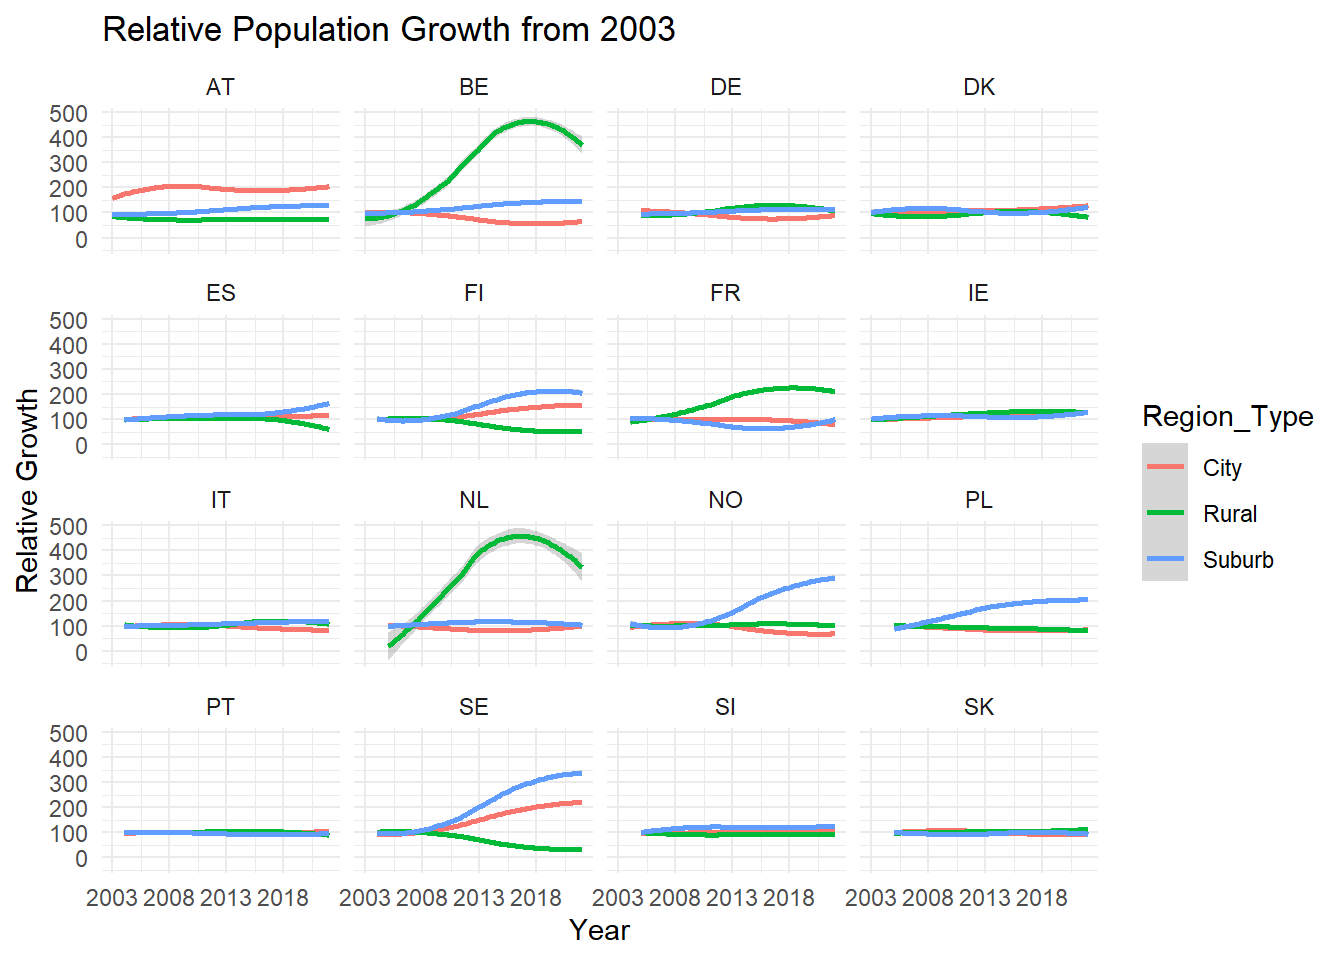
\includegraphics{assignment_files/figure-pdf/fig-9-1.pdf}

}

\caption{\label{fig-9}Relativ populasjonsvekst gruppert etter land}

\end{figure}

\hypertarget{section}{%
\subsection{}\label{section}}

\begin{Shaded}
\begin{Highlighting}[]
\NormalTok{merged }\SpecialCharTok{|\textgreater{}} 
  \FunctionTok{filter}\NormalTok{(}
    \FunctionTok{str\_sub}\NormalTok{(Country, }\AttributeTok{start =}\NormalTok{ 1L, }\AttributeTok{end =}\NormalTok{ 2L) }\SpecialCharTok{\%in\%} \FunctionTok{c}\NormalTok{( }\StringTok{"PL"}\NormalTok{, }\StringTok{"PT"}\NormalTok{, }\StringTok{"SI"}\NormalTok{, }\StringTok{"SK"}\NormalTok{)}
\NormalTok{  ) }\SpecialCharTok{|\textgreater{}} 
    \FunctionTok{filter}\NormalTok{(Year }\SpecialCharTok{\textgreater{}=} \DecValTok{2005}\NormalTok{) }\SpecialCharTok{|\textgreater{}} 
  \FunctionTok{ggplot}\NormalTok{(}
    \FunctionTok{aes}\NormalTok{(}
      \AttributeTok{x =}\NormalTok{ Year,}
      \AttributeTok{y =}\NormalTok{ Relative\_Growth,}
      \AttributeTok{group =}\NormalTok{ Class,}
      \AttributeTok{color =} \FunctionTok{as.factor}\NormalTok{(Class)}
\NormalTok{    )}
\NormalTok{  ) }\SpecialCharTok{+}
  \FunctionTok{geom\_smooth}\NormalTok{(}\AttributeTok{span =} \DecValTok{1}\NormalTok{, }\AttributeTok{se =} \ConstantTok{FALSE}\NormalTok{) }\SpecialCharTok{+}
  \FunctionTok{xlim}\NormalTok{(}\DecValTok{2005}\NormalTok{, }\DecValTok{2022}\NormalTok{)  }
\end{Highlighting}
\end{Shaded}

\begin{verbatim}
`geom_smooth()` using method = 'loess' and formula = 'y ~ x'
\end{verbatim}

\begin{figure}[H]

{\centering 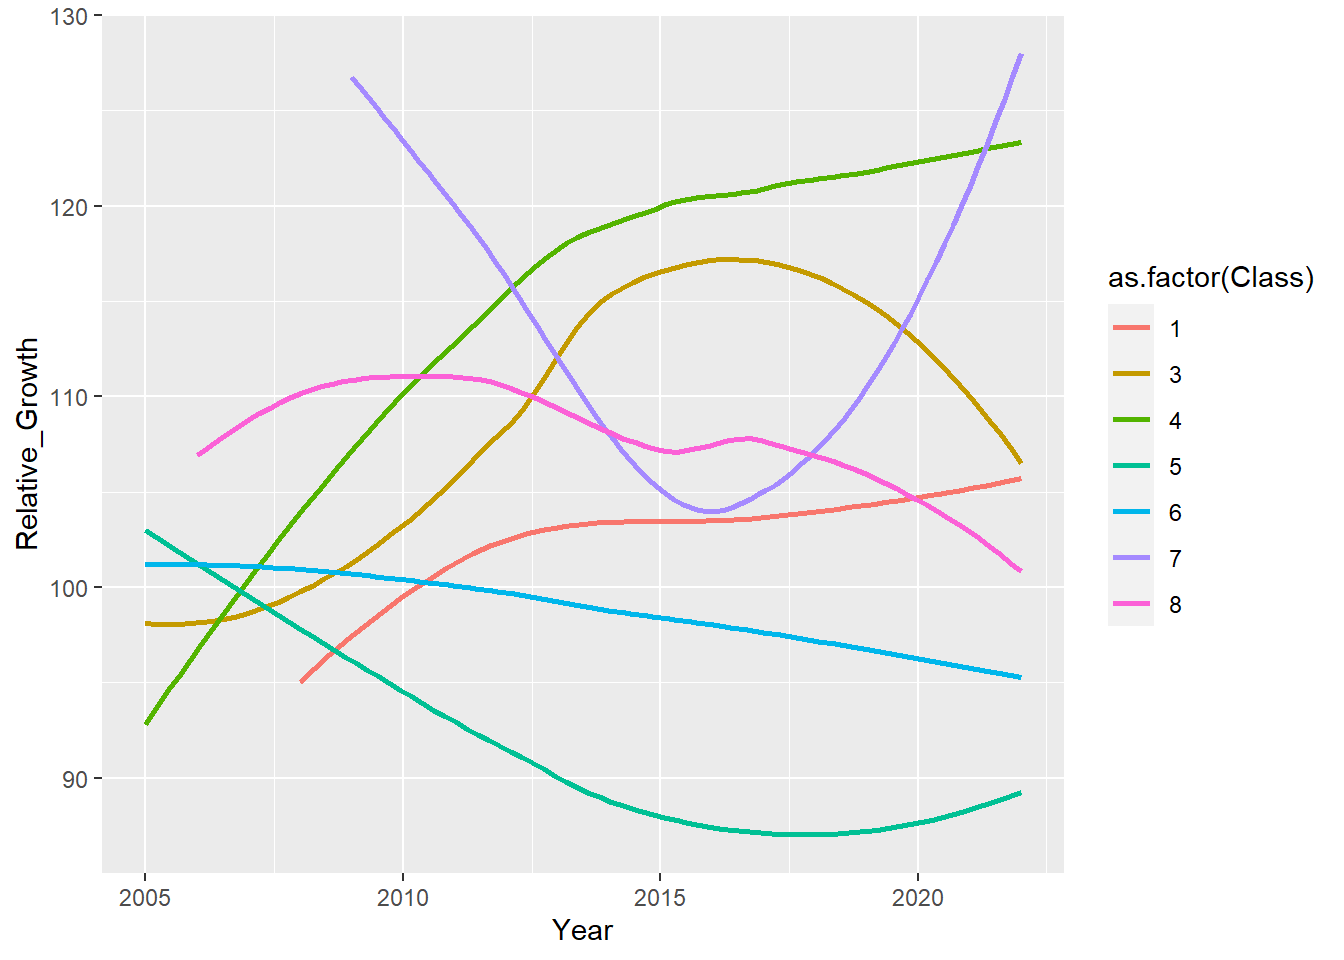
\includegraphics{assignment_files/figure-pdf/unnamed-chunk-29-1.pdf}

}

\end{figure}

\begin{figure}

{\centering 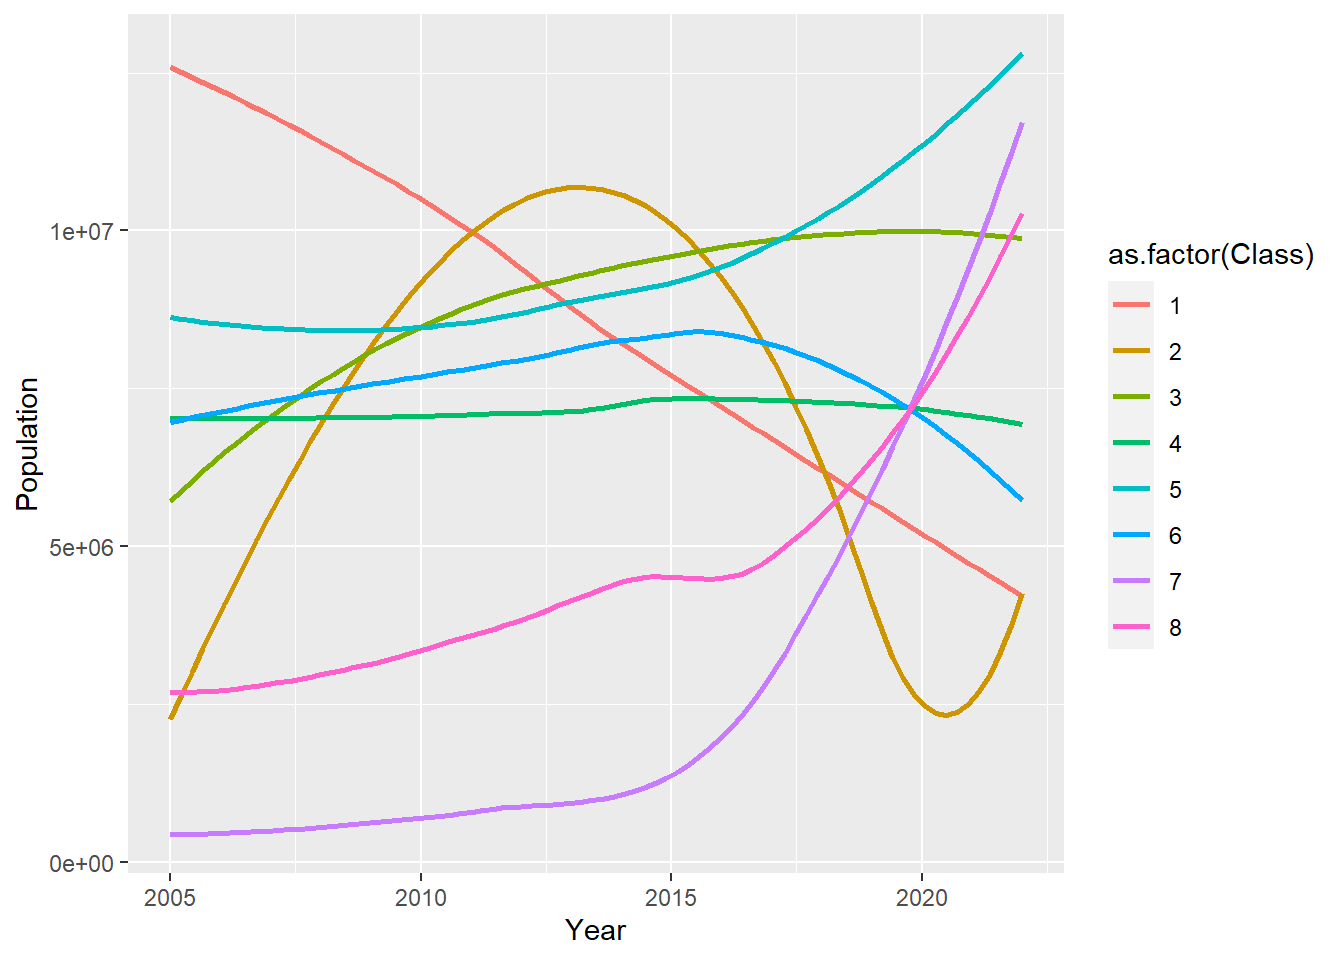
\includegraphics{assignment_files/figure-pdf/fig-8-1.pdf}

}

\caption{\label{fig-8}Populasjonsvekst i de 8 forskjellige gruppene}

\end{figure}

\hypertarget{refs}{}
\begin{CSLReferences}{1}{0}
\leavevmode\vadjust pre{\hypertarget{ref-andersson2019b}{}}%
Andersson, Magnus, Peter G. Håkansson, and Inge Thorsen. 2019.
{``Centralization and {Urbanization Tendencies} in {Norway}.''} In
\emph{Investigating {Spatial Inequalities}}, edited by Peter Gladoić
Håkansson and Helena Bohman, 31--54. {Emerald Publishing Limited}.

\leavevmode\vadjust pre{\hypertarget{ref-capello2015}{}}%
Capello, Roberta. 2015. \emph{Regional {Economics}}. 2nd ed. {London}:
{Routledge}.

\leavevmode\vadjust pre{\hypertarget{ref-christiansen2011}{}}%
Christiansen, Petter, and Tanja Loftsgarden. 2011. \emph{Drivers Behind
Urban Sprawl in {Europe}}.

\leavevmode\vadjust pre{\hypertarget{ref-zotero-187}{}}%
{``Database - {Eurostat}.''} n.d.
https://ec.europa.eu/eurostat/data/database. Accessed February 14, 2024.

\leavevmode\vadjust pre{\hypertarget{ref-detoni2021}{}}%
De Toni, Andrea, Paolo Di Martino, and Thomas Dax. 2021. {``Location
Matters. {Are} Science and Policy Arenas Facing the {Inner Peripheries}
Challenges in {EU}?''} \emph{Land Use Policy} 100 (January): 105111.

\leavevmode\vadjust pre{\hypertarget{ref-europeancommission.statisticalofficeoftheeuropeanunion.2021}{}}%
European Commission. Statistical Office of the European Union. 2021.
\emph{Applying the Degree of Urbanisation: A Methodological Manual to
Define Cities, Towns and Rural Areas for International Comparisons :
2021 Edition.} {LU}: {Publications Office}.

\leavevmode\vadjust pre{\hypertarget{ref-moreno-llamas2021}{}}%
Moreno-Llamas, Antonio, Jesús García-Mayor, and Ernesto De la
Cruz-Sánchez. 2021. {``Urban-Rural Differences in Trajectories of
Physical Activity in {Europe} from 2002 to 2017.''} \emph{Health \&
Place} 69 (May): 102570.

\leavevmode\vadjust pre{\hypertarget{ref-wolff2018}{}}%
Wolff, Manuel. 2018. {``Understanding the Role of Centralization
Processes for Cities {\textendash} {Evidence} from a Spatial Perspective
of Urban {Europe} 1990{\textendash}2010.''} \emph{Cities} 75 (May):
20--29.

\end{CSLReferences}



\end{document}
